% Chapter 2 -- Financial Data and How to Use It Well
% Requires: amsmath, amssymb, booktabs, array, tabularx, longtable, graphicx, tcolorbox (breakable, skins), hyperref or url.
% Defines the callout box only if the preamble has not.
\providecolor{fenavy}{HTML}{1B2A6B}
\providecolor{feshade}{HTML}{F3F5FA}
\makeatletter
\@ifundefined{callout}{%
  \newtcolorbox{callout}{breakable, enhanced,
    colback=white, colframe=gray!70, boxrule=0.5pt, arc=1mm,
    borderline west={2.5pt}{0pt}{gray!70},
    left=8pt, right=8pt, top=4pt, bottom=4pt}%
}{}
\makeatother

\chapter{Financial Data and How to Use It Well}
\label{ch:02}

Chapter~\ref{ch:01} showed what a track record must do to reveal real skill. This chapter turns to something that comes before any track record, namely the data on which it is built. A backtest\index{backtest} can test a single idea with honest statistics and still give the wrong answer because of the way its dataset was put together. Fortunately, each of these problems is well understood, and each one has a fix.

The problems are rarely dramatic. Each one looks like a small technical detail, yet each can add a percentage point or more a year to a strategy's measured return. The most common are the following:

\begin{itemize}
  \item a price series that is not adjusted for stock splits and dividends, so that ordinary corporate events look like gains or losses;
  \item a portfolio that gives a \$20 million company the same weight as a \$2 trillion one, so that the result is driven by stocks that almost no one can trade in size;
  \item a database that keeps only the companies that still exist, so that the failures, and the losses they caused, are missing;
  \item an accounting number that is used months before it was published, so that the strategy trades on information no investor had at the time;
  \item an average return that is quoted in a way that overstates what an investor actually earned.
\end{itemize}

The claim on trial\index{claims-on-trial method} in this chapter is one that every reader who works with free data needs to be true: \textbf{free, public data can support a reliable backtest.} Because every lab in this book relies on this claim, we test it first, and the answer comes with a checklist that shows you how to make it true in your own work.


By the end of the chapter you will be able to:

\begin{itemize}
  \item explain how stock splits and dividends change quoted prices, and why research uses adjusted prices\index{data!adjusted prices};
  \item compute market capitalization\index{market capitalization} and distinguish value-weighted\index{index weighting!value-weighted}, equal-weighted\index{index weighting!equal-weighted} and price-weighted\index{index weighting!price-weighted} portfolios;
  \item describe the main research datasets and their free counterparts, and explain delisting returns\index{return!delisting} and point-in-time\index{data!point-in-time} data;
  \item choose the right return measure for each task (simple or log, price or total, raw or excess), and explain why arithmetic and geometric averages\index{geometric average} differ;
  \item recognize survivorship bias\index{survivorship bias}, look-ahead bias\index{look-ahead bias}, micro-cap\index{micro-caps} effects and data snooping\index{data snooping}, and estimate how much each can distort a result;
  \item apply a data checklist before trusting any backtest.
\end{itemize}

In the lab you will use nearly a century of real market data, together with one controlled simulation, to measure four of these problems. You will see how much each problem can inflate a strategy's apparent performance and how much of that inflation\index{inflation} each fix removes.

\section{Foundations: where financial data comes from}
\label{sec:02-foundations}

\subsection{Prices, corporate actions and adjusted prices}

A stock's quoted price can change for reasons that bring shareholders neither a gain nor a loss. The events that cause such changes are called \textbf{corporate actions}\index{corporate actions|textbf}, and two of them matter most.

\begin{itemize}
  \item \textbf{Stock split.} In a two-for-one split, each share becomes two shares and the price is cut in half. A shareholder who owned one share worth \$100 now owns two shares worth \$50 each, so the holding is still worth \$100. A chart of the raw price, however, would show a 50\% ``crash'' that never cost anyone a cent.
  \item \textbf{Dividend.} A dividend is a cash payment that a company makes to its shareholders. Only investors who own the stock before the \emph{ex-dividend date} receive the payment, and anyone who buys on or after that date does not. For this reason, the share price usually falls by about the amount of the dividend on the ex-dividend date. Suppose, for example, that a \$100 stock pays a \$2 dividend and opens at \$98 on the ex-dividend date. The price return is $-2$\%, but the shareholder has lost nothing, because they now hold \$98 in stock and \$2 in cash, so their total return\index{return!total} is zero.
\end{itemize}

Databases therefore publish \textbf{adjusted prices}\index{data!adjusted prices|textbf}, which rescale past prices so that the change in the adjusted price equals the return a shareholder actually earned. After the split above, for example, every earlier price is divided by two. Total-return series go one step further and also adjust for dividends. Data vendors do not all make these adjustments in the same way, which is one reason why two sources can disagree about the history of the same stock.

\subsection{Market capitalization and index weights}

A company's \textbf{market capitalization}\index{market capitalization|textbf}, or market value, is its share price multiplied by the number of shares outstanding, so a company with one billion shares priced at \$50 is worth \$50 billion. The way a portfolio uses this number determines which stocks drive its results, and there are three common approaches.

\begin{itemize}
  \item A \textbf{value-weighted}\index{index weighting!value-weighted|textbf} (or capitalization-weighted) portfolio holds each stock in proportion to its market capitalization. If company A is worth \$900 billion and company B is worth \$100 billion, the two are worth \$1 trillion together, so A receives 90\% of the money invested and B receives 10\%.
  \item An \textbf{equal-weighted}\index{index weighting!equal-weighted|textbf} portfolio puts the same amount of money into each stock, whatever its size, so A and B would each receive 50\%. Because company B makes up only 10\% of the market's value but receives half of the portfolio, equal weighting\index{equal weighting (1/N)} gives small companies far more influence than their size in the economy would justify.
  \item A \textbf{price-weighted}\index{index weighting!price-weighted|textbf} index, such as the Dow Jones Industrial Average, weights each stock by its share price alone. A \$500 stock therefore counts ten times as much as a \$50 stock, regardless of how large the two companies are. This method is a historical convention and has no economic justification.
\end{itemize}

A value-weighted portfolio needs little rebalancing\index{rebalancing}, because its weights move with prices automatically. It trades mainly when stocks enter or leave the portfolio, or when companies issue new shares or buy back existing ones. An equal-weighted portfolio, by contrast, must be rebalanced regularly as prices drift apart, which means selling part of the stocks that have risen and buying more of those that have fallen until the weights are equal again.


\subsection{The main research databases}

Most empirical research in finance rests on a small number of data sources, which are summarized in the table below.

\begingroup
\small
\setlength{\LTpre}{6pt}\setlength{\LTpost}{6pt}
\begin{longtable}{@{}>{\raggedright\arraybackslash}p{0.2\linewidth}>{\raggedright\arraybackslash}p{0.42\linewidth}>{\raggedright\arraybackslash}p{0.22\linewidth}@{}}
\toprule
Source & What it holds & Access \\
\midrule
\endfirsthead
\multicolumn{3}{@{}l}{\emph{(continued)}}\\
\toprule
Source & What it holds & Access \\
\midrule
\endhead
\midrule
\multicolumn{3}{r@{}}{\emph{continued on next page}}\\
\endfoot
\bottomrule
\endlastfoot
CRSP (Center for Research in Security Prices) & Daily and monthly returns, prices, shares and delisting information for U.S. stocks since 1926, including companies that no longer exist & Subscription, usually through WRDS \\
Compustat & Company accounting data: balance sheets, income statements, cash flows & Subscription \\
Kenneth R. French Data Library & Factor returns and sorted portfolio returns built from CRSP and Compustat & Free \\
FRED (Federal Reserve Bank of St.\ Louis) & Interest rates, inflation, macroeconomic series; ALFRED holds earlier vintages & Free \\
Exchange and vendor feeds (Yahoo Finance and others) & Recent prices and adjusted prices for currently listed securities & Free or commercial; coverage and adjustment methods vary \\
\end{longtable}
\endgroup

Most universities access CRSP\index{CRSP} and Compustat\index{Compustat} through WRDS (Wharton Research Data Services), a subscription platform.

Two terms in the table need explaining. A \textbf{factor} is the return on a portfolio that is designed to track one source of return. The size factor, for example, buys small companies and sells large ones, so its return measures how much small companies have beaten, or trailed, large ones. A \textbf{vintage}\index{data!vintages|textbf} is a dataset as it looked on a particular date, before any later corrections were made. All the labs in this book use free data, and when a test needs data that only paid databases provide, such as the returns of companies that stopped trading, the lab uses simulated data instead.

\subsection{Delisting}

A company is \textbf{delisted}\index{delisting|textbf} when its stock stops trading on an exchange, which can happen because the company is bought by another firm, goes private, moves to a different exchange or fails. The \textbf{delisting return}\index{return!delisting|textbf} measures the change from the stock's last trading price to the amount that shareholders finally receive. When a company fails, this return can be a large loss, since shareholders may receive only a few cents a share or nothing at all. A database that drops delisted companies, or that leaves out their final return, misses these losses and makes past returns look better than they really were.


\subsection{Dates and timing}

Companies report their accounting results for a \textbf{fiscal year}\index{fiscal year|textbf}, which is a twelve-month reporting period that does not always end in December. These results are published weeks or months after the year ends, so a company whose fiscal year ends on 31 December may not release its annual report until February or March. A study that treats the figures as known on the last day of the fiscal year, rather than on the day they were published, gives itself information that no investor actually had at the time. \textbf{Point-in-time}\index{data!point-in-time|textbf} data avoids this problem by recording what was known on each date, including the original values of any numbers that were later revised.

\section{Measuring returns: choosing the right measure}
\label{sec:02-returns}

Every claim in this book is ultimately a statement about returns, so the way a return is measured determines what the claim actually says. The same investment can produce quite different numbers depending on whether dividends are included, whether the risk-free rate\index{risk-free rate} is subtracted and how the returns are averaged. If you choose the wrong measure, a strategy can appear to beat the market by several percentage points a year without earning anything extra.

Section~\ref{sec:01-foundations} defined the simple return\index{return!simple} (Equation~\eqref{eq:01-return}), the log return\index{return!log}, total and price returns, and excess returns\index{return!excess}. This section explains which of these measures to use for each task, and four rules cover most cases.

\textbf{Use simple returns across assets and log returns across time.} Section~\ref{sec:01-foundations} showed that log returns add up over time, whereas simple returns compound. The two measures also differ in the direction in which they add up.

\begin{itemize}
  \item \textbf{Simple returns add across assets.} A portfolio's simple return is the weighted average of the simple returns of its holdings. If half the money earns 10\% and the other half earns 2\%, the portfolio earns 6\%.
  \item \textbf{Log returns add across time.} The log return over several periods is the sum of the log returns of the individual periods, so log returns of 5\% and 3\% add up to 8\% over the two periods.
\end{itemize}

You should therefore use simple returns when you build portfolios and log returns when you compound over time or use certain statistical models, and you should never mix the two in one calculation.

\textbf{Compare total return with total return.} A total return includes dividends, whereas a price return does not (Section~\ref{sec:01-foundations}). Over long periods the difference is large, because dividends have supplied a substantial share of U.S. stock market returns over the past century. Many free sources, including most stock charts, nevertheless show price indexes. If you compare a strategy's total return with an index's price return, the strategy will look better than it really is, because it will appear to beat the index by the \textbf{dividend yield}\index{valuation ratios!dividend yield|textbf}, which is the annual dividend divided by the price, even when it has no real advantage. Before comparing any two returns, you should therefore check that both include dividends.

\textbf{Judge a strategy by its excess return.} Performance should be measured as the return above the risk-free rate (Section~\ref{sec:01-foundations}) rather than as the raw return. A strategy that earned 5\% in a year when Treasury bills also paid 5\% added nothing in exchange for the risk it took. Because the Sharpe ratio\index{Sharpe ratio} and the regressions in later chapters all use excess returns, it is best to compute them from the start.

\textbf{Quote the geometric average when reporting what an investor earned.} There are two ways to average a series of returns, and they answer different questions.

\begin{itemize}
  \item The \textbf{arithmetic average}\index{arithmetic average|textbf}, $A$, is the simple mean of the period returns, and it estimates the expected return\index{return!expected} in any single period.
  \item The \textbf{geometric average}\index{geometric average|textbf}, $G$, is the constant rate of return that would have produced the same ending wealth, so it describes what a buy-and-hold investor actually earned:
  \begin{equation}
    G = \left(\prod_{t=1}^{T} (1 + R_t)\right)^{1/T} - 1
    \label{eq:02-geometric}
  \end{equation}
\end{itemize}

A simple example shows why the choice matters. Suppose an investment gains 50\% in one year and loses 50\% in the next. The arithmetic average is $(50 - 50)/2 = 0$\%, which sounds like breaking even. In fact, \$100 grows to \$150 in the first year and then falls to \$75 in the second, so the investor has lost a quarter of the money. The geometric average, $\sqrt{1.5 \times 0.5} - 1 \approx -13.4$\% a year, matches what actually happened.

Whenever returns vary, the geometric average is lower than the arithmetic average, and the gap between them grows with volatility\index{volatility}. This gap is often called \textbf{volatility drag}\index{volatility drag|textbf}, and it can be estimated with a useful approximation:
\begin{equation}
  G \approx A - \frac{\sigma^2}{2}
  \label{eq:02-drag}
\end{equation}
where $\sigma$ is the volatility. For a stock index with 20\% annual volatility, the gap is about $0.20^2/2 = 0.02$, or 2 percentage points a year, while for a portfolio of small, volatile stocks with 35\% volatility it is about 6 percentage points (Figure~\ref{fig:02-drag}).

%\begin{figure}[htbp]
%\centering
%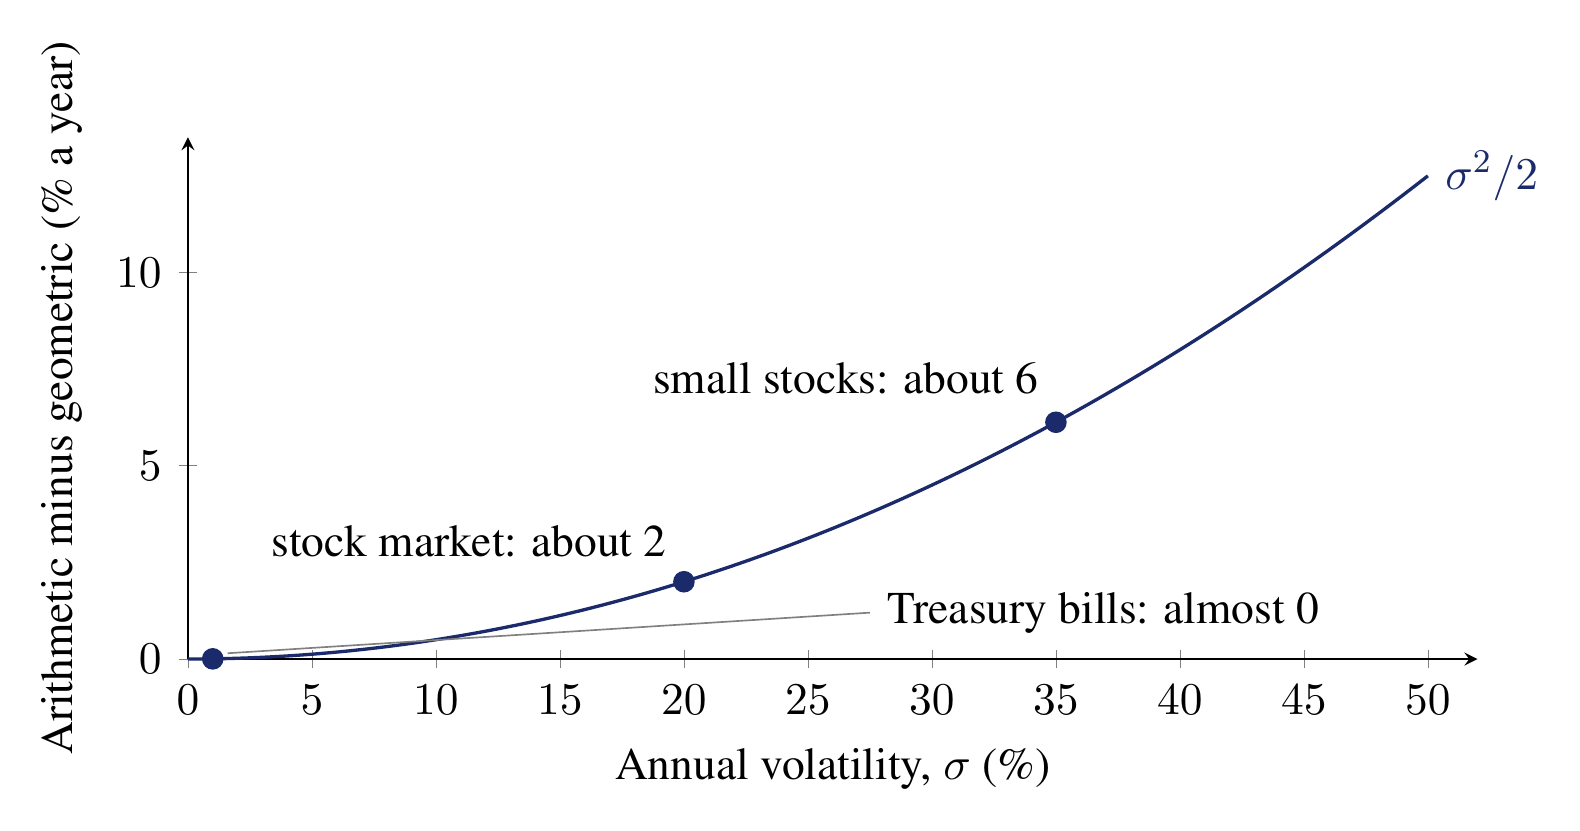
\includegraphics[width=0.85\linewidth]{images/fig02-1-volatility-drag.png}
%\caption{Volatility drag: the gap between the arithmetic and geometric average returns, from Equation~\eqref{eq:02-drag}. The gap is negligible for Treasury bills, about 2 percentage points a year for the stock market and about 6 for small stocks, and it rises with the square of volatility.}
%\label{fig:02-drag}
%\end{figure}


\providecolor{fenavy}{HTML}{1B2A6B}

\begin{figure}[!htbp]
  \centering
  \begin{tikzpicture}[
    % Arithmetic minus geometric mean = sigma^2 / 2.
    % With sigma in percent: (sigma/100)^2 / 2 * 100 = sigma^2 / 200 (% a year).
    declare function={gap(\s) = \s^2/200;}
  ]
  \begin{axis}[
    scale only axis, width=0.55\linewidth, height=0.28\linewidth,
    axis lines=left,
    axis line style={-stealth, thin},
    xmin=0, xmax=52, ymin=0, ymax=14,
    xtick={0,10,...,50},
    ytick={0,5,10},
    tick label style={font=\small},
    label style={font=\small},
    xlabel={Annual volatility, $\sigma$ (\%)},
    ylabel={Arith.\ minus geom.\ (\% a year)},
    samples=150, domain=0:50,
    clip=false,
  ]
    \addplot[fenavy, thick] {gap(x)};
    \node[fenavy, anchor=west, font=\small] at (axis cs:50.3,{gap(50)}) {$\sigma^2/2$};

    % Examples
    \fill[fenavy] (axis cs:1,{gap(1)})   circle (2pt);
    \fill[fenavy] (axis cs:20,{gap(20)}) circle (2pt);
    \fill[fenavy] (axis cs:35,{gap(35)}) circle (2pt);

    \node[anchor=south east, font=\footnotesize] at (axis cs:19.5,{gap(20)+0.2}) {stock market: about 2};
    \node[anchor=south east, font=\footnotesize] at (axis cs:34,{gap(35)+0.3}) {small stocks: about 6};
    \draw[gray!60] (axis cs:1.5,0.15) -- (axis cs:27,1.3);
    \node[anchor=west, font=\footnotesize] at (axis cs:27,1.4) {Treasury bills: almost 0};
  \end{axis}
  \end{tikzpicture}
  \caption{Volatility drag: the gap between the arithmetic and geometric average returns, from Equation~\eqref{eq:02-drag}. The gap is negligible for Treasury bills, about 2 percentage points a year for the stock market and about 6 for small stocks, and it rises with the square of volatility.}
  \label{fig:02-drag}
\end{figure}

\textbf{Implications:}
\begin{enumerate}
\item Use the arithmetic average when you need the expected return for a single period, as in the Sharpe ratio or a forecast, and use the geometric average when you report how much an investment grew. 
\item If you quote the arithmetic average as a growth rate, you will overstate what the investor experienced, and the overstatement is largest for the volatile strategies that tend to look most attractive. 
\item Whenever a source reports an average return, you should check which kind it is. Lab~\ref{ch:02} measures the gap on real portfolios.
\end{enumerate}

\section{Research datasets and their free alternatives}
\label{sec:02-datasets}

A result can be no more reliable than the data behind it. Each dataset covers different companies, periods and events, and each handles corrections, dividends and failed companies in its own way. 

Most published research on U.S. stocks rests on CRSP and Compustat, the two commercial databases introduced in Section~\ref{sec:02-foundations}. Two of their features\index{features and targets} matter most for this chapter, because free sources usually lack them.

\begin{itemize}
  \item \textbf{Delisting returns.}\index{return!delisting|textbf} CRSP includes companies that later disappeared, together with the return in the month in which each of them was delisted.
  \item \textbf{Point-in-time data.}\index{data!point-in-time|textbf} The point-in-time version of Compustat records what was known on each date, rather than the figures as they were later revised.
\end{itemize}

Many universities subscribe to these databases, but many readers will not have access to them. The labs in this book therefore use free sources that are either built from these databases or comparable to them:

\begin{center}
\small
\begin{tabularx}{0.9\linewidth}{@{}>{\raggedright\arraybackslash}p{0.22\linewidth}>{\raggedright\arraybackslash}X>{\raggedright\arraybackslash}p{0.26\linewidth}@{}}
\toprule
Free source & What it offers & Main limitation \\
\midrule
Kenneth R. French Data Library & Factor returns and portfolios sorted on size, value, momentum and more, built from CRSP and Compustat, since 1926 & Portfolio-level only; no individual stocks \\
FRED (Federal Reserve Bank of St.\ Louis) & Interest rates and economic series; its ALFRED archive keeps past vintages of revised data & Economic series, not stock-level data \\
Open Source Asset Pricing (Chen and Zimmermann) & Portfolio returns for over 200 published predictors & Full firm-level signals require WRDS \\
Jensen--Kelly--Pedersen global factors & 153 factors across 93 countries & Factor-level only \\
Yahoo Finance and similar & Daily prices for current stocks, ETFs and indexes & Mostly survivors only; adjustments not always documented; unofficial access methods can break \\
\bottomrule
\end{tabularx}
\end{center}

A \textbf{predictor}, also called a \textbf{signal}, is a variable that a study uses to forecast returns, such as a valuation ratio or a past return. The last row of the table deserves particular attention. Free stock-price sites are convenient, but they mostly cover companies that still exist today. A backtest that downloads today's stocks from such a site and runs them through the past therefore has survivorship bias built into it, which is the problem that Section~\ref{sec:02-survivorship} describes.

\section{Survivorship bias: the missing failures}
\label{sec:02-survivorship}

Companies that fail, merge or are delisted disappear from many datasets, and their final losses disappear with them. A backtest that is run only on companies that still exist never suffers those losses, so it overstates returns, often by several percentage points a year. This is one of the most common errors in practice, because most free price sources list only the stocks that trade today.

\subsection{Survivorship bias}

\textbf{Survivorship bias}\index{survivorship bias|textbf} arises when a sample includes only the companies, funds or strategies that are still around at the end of the period. Those that failed, were acquired or were shut down drop out of the data, and their losses drop out with them. It is like judging how safe a sport is by interviewing only the players who are still playing.

The bias works through three channels.

\begin{enumerate}
  \item \textbf{Survivors-only samples.} Testing a strategy on today's index members, or on the funds that exist today, removes every company or fund that failed along the way. The survivors are, by definition, the ones that did well enough to last.
  \item \textbf{Missing delisting returns.} When a stock leaves the exchange because the company is failing, its final return is often large and negative, and it is often missing from the database. Shumway (1997) showed that CRSP frequently lacked returns for delistings caused by poor performance, and he estimated that these missing returns averaged about $-30$\% for stocks on the NYSE and AMEX. Shumway and Warther (1999) found even larger losses for Nasdaq stocks. A backtest that silently drops these months overstates returns, and the error is largest for small and distressed stocks.
  \item \textbf{Backfill.}\index{backfill bias|textbf} Databases sometimes add a company or fund only after it has already succeeded, filling in its earlier history at the same time. This \textbf{backfill} brings in past returns only for those that did well. Kothari, Shanken and Sloan (1995) argued that this kind of selection in Compustat inflated the measured returns of high book-to-market\index{book-to-market ratio} stocks, which are companies whose accounting value is large relative to their market value.
\end{enumerate}

The bias is well documented for mutual funds. Elton, Gruber and Blake (1996) estimated that studying only the funds that survived overstated average performance by roughly 0.9 percentage points a year, which is large compared with the alphas\index{alpha} that researchers try to detect. Brown, Goetzmann, Ibbotson and Ross (1992) showed that survivorship can even make fund performance appear to persist from one period to the next when in fact it does not.

\subsection{The problem}

\textbf{Why survivorship can create a strategy out of nothing.} Survivorship bias does not simply shift all returns upward by the same amount. Its effect is strongest for the stocks that are most likely to fail, namely small, volatile and \textbf{distressed} companies that are at real risk of bankruptcy. Among such companies, the ones that survive are the ones whose prices happened to rise. As a result, a survivors-only backtest of a strategy that buys volatile or distressed stocks can show a large premium that is produced entirely by the way the sample was built. Lab~\ref{ch:02} demonstrates this with a simulation in which the true premium is known to be zero.

\subsection{The fix}

\textbf{The fix} is to use a dataset that includes failed companies and their delisting returns, such as CRSP, together with portfolio rules that use only the firms that were listed on each date. 
Most free sources in Section~\ref{sec:02-datasets} do not need this fix. The French library, Open Source Asset Pricing\index{Open Source Asset Pricing} and the Jensen--Kelly--Pedersen data are built from CRSP, so they include companies that later failed, and FRED\index{FRED} holds economic series rather than companies. The fix matters most for free stock-price sites such as Yahoo Finance, which list mainly today's survivors. Because those sites do not show which companies are missing, the Shumway correction cannot be applied, and the safer choice is to test the strategy on portfolio data that were built from a complete database.

When delisting returns are missing, researchers follow Shumway and substitute an estimate, such as $-30$\%.
Suppose a stock falls from \$10 to \$2 and is then delisted for poor performance, with no final return recorded.
If the final return is left blank, the backtest counts only the fall to \$2.
If the researcher follows Shumway, the backtest adds one more month with a $-30$\% return, as if the stock ended near \$1.40.
The estimate won’t be exact for any single company, but on average it is much closer to the truth than assuming a zero loss.
Do we need to do this fix? Probably not. Only researchers with stock-level data such as CRSP can apply it, because they can see which companies were delisted and which delisting returns are missing. Users of Yahoo Finance can’t, because the failed companies aren’t in the data at all.


\section{Look-ahead bias: using only what was known}
\label{sec:02-lookahead}

A backtest is honest only if every decision in it uses information that was available at the time. Accounting figures are published weeks or months after the period they describe, and economic data are often revised later. Using the final numbers as if they had been known in advance gives a strategy an advantage that no investor had, and the result can look excellent for no real reason.

\textbf{Look-ahead bias}\index{look-ahead bias|textbf} arises when a backtest uses information that was not yet available when the decision would have been made. It is easy to introduce and hard to notice, because the code runs without error and the results simply look better than they should. Figure~\ref{fig:02-timeline} shows the most common case, in which accounting data are used before they were published.

%\begin{figure}[htbp]
%\centering
%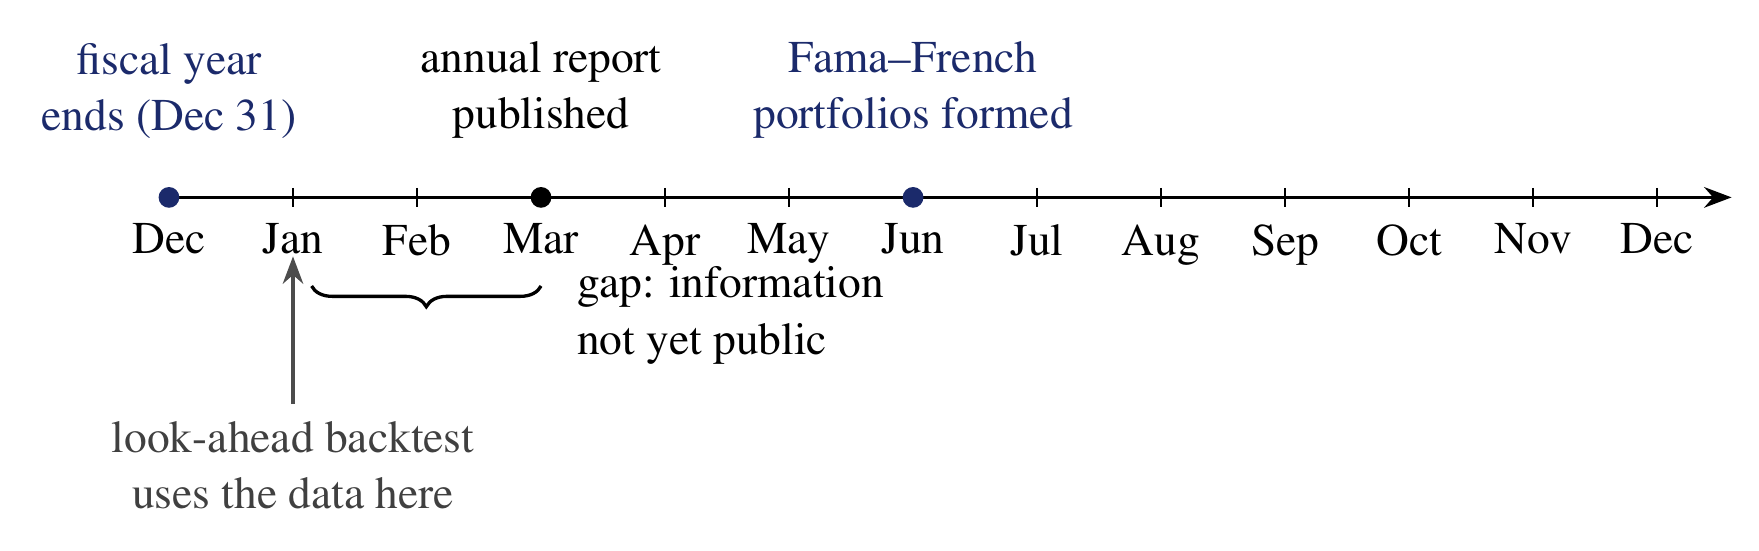
\includegraphics[width=0.9\linewidth]{images/fig02-2-accounting-timeline.png}
%\caption{When accounting data becomes usable. A company's fiscal year ends in December, but its annual report appears only months later. A backtest that trades on the figures in January uses information no investor had. Fama and French wait until the following June to be safe.}
%\label{fig:02-timeline}
%\end{figure}

\providecolor{fenavy}{HTML}{1B2A6B}
\providecolor{fegray}{HTML}{4D4D4D}

\begin{figure}[!htbp]
  \centering
  \begin{tikzpicture}[x=0.9cm, y=1cm, font=\small]
    % Timeline: Dec (0) to the following Dec (12)
    \draw[-stealth, thick] (0,0) -- (12.6,0);
    \foreach \wfI/\wfM in {0/Dec,1/Jan,2/Feb,3/Mar,4/Apr,5/May,6/Jun,
                           7/Jul,8/Aug,9/Sep,10/Oct,11/Nov,12/Dec} {
      \draw (\wfI,0.1) -- (\wfI,-0.1);
      \node[anchor=north] at (\wfI,-0.12) {\wfM};
    }

    % Key dates
    \fill[fenavy] (0,0) circle (2.6pt);
    \fill         (3,0) circle (2.6pt);
    \fill[fenavy] (6,0) circle (2.6pt);
    \node[fenavy, anchor=south, align=center] at (0,0.3)
      {fiscal year\\ends (Dec 31)};
    \node[anchor=south, align=center] at (3,0.3)
      {annual report\\published};
    \node[fenavy, anchor=south, align=center] at (6,0.3)
      {Fama--French\\portfolios formed};

    % Gap between fiscal year-end and publication
    \draw[decorate, decoration={brace, mirror, amplitude=5pt}]
      (1.1,-0.65) -- (2.9,-0.65);
    \node[anchor=north west, align=left] at (3.1,-0.5)
      {gap: information\\not yet public};

    % Look-ahead bias
    \draw[-stealth, fegray] (1,-1.9) -- (1,-0.6);
    \node[fegray, anchor=north, align=center] at (1,-2)
      {look-ahead backtest\\uses the data here};
  \end{tikzpicture}
\caption{When accounting data becomes usable. A company's fiscal year ends in December, but its annual report appears only months later. A backtest that trades on the figures in January uses information that no investor had, which is why Fama and French wait until the following June.}
\label{fig:02-timeline}
\end{figure}


The table below lists the common sources of look-ahead bias and the standard treatment against each.

\begin{center}
\small
\begin{tabularx}{0.9\linewidth}{@{}r>{\raggedright\arraybackslash}p{0.16\linewidth}>{\raggedright\arraybackslash}X>{\raggedright\arraybackslash}p{0.32\linewidth}@{}}
\toprule
 & Source & What goes wrong & Standard treatment \\
\midrule
1 & Same-period execution & A signal computed from today's closing price is used to trade at that same close & Trade on the next period's return: lag every signal by at least one period \\
2 & Accounting publication lags & Annual results for a December fiscal year are used in January, though they are published weeks or months later & Lag accounting data; Fama and French (1993) use fiscal-year data only from the following June \\
3 & Revised economic data & GDP or employment figures are used as revised years later, not as first reported & Use real-time vintages, such as FRED's ALFRED archive \\
4 & Index membership & Today's index members are used for the past & Use historical membership lists \\
5 & Full-sample choices & Parameters, thresholds or variable definitions are chosen using the whole sample, then ``tested'' on it & Choose using only data available at each date (walk-forward; Chapter~\ref{ch:05}) \\
6 & Full-sample scaling & Signals are standardized with means and volatilities computed over the whole sample & Use expanding or rolling estimates \\
\bottomrule
\end{tabularx}
\end{center}


Three terms in the table need explaining. To \textbf{lag} a signal is to use it only from a later period, so that it was already known before the trade. A \textbf{walk-forward}\index{walk-forward evaluation|textbf} test chooses its settings at each date using only the data available before that date, just as an investor in real time would have to. An \textbf{expanding} estimate uses all the data up to each date, whereas a \textbf{rolling} estimate uses a window of fixed length, such as the past five years.

The last two rows of the table describe the subtlest problems. In these cases no future price is used directly, yet the analyst's choices reflect knowledge of how the whole period turned out. For example, a trading rule whose window length was chosen because it worked best over 1926--2025 carries information from 2025 back into 1926.

\textbf{Point-in-time data}\index{data!point-in-time|textbf} is the general remedy, because it ensures that each date uses only the values that could have been known then. Lab~\ref{ch:02} measures two forms of look-ahead bias on real data, namely trading on the same day's closing price and choosing a rule's parameter with hindsight.

\section{Micro-caps: results no investor could capture}
\label{sec:02-microcaps}

The smallest companies are costly or impossible to trade in large amounts, yet in an equal-weighted portfolio they carry the same weight as the largest companies. A result can therefore be driven almost entirely by stocks that no investor could realistically buy. Checking how a portfolio is weighted, and whether its result survives without the smallest stocks, is one of the quickest ways to test whether a finding is usable.

The U.S. stock market is extremely unequal. A few hundred large companies account for most of its value, while thousands of tiny companies account for most of the names on the list. Fama and French (2008) classified stocks below the 20th percentile of NYSE market capitalization as \textbf{micro-caps}\index{micro-caps|textbf}, which means that each of them is smaller than four-fifths of the stocks listed on the New York Stock Exchange. They found that micro-caps made up about 60\% of all listed stocks but only about 3\% of total market value (Figure~\ref{fig:02-microcaps}).

%\begin{figure}[htbp]
%\centering
%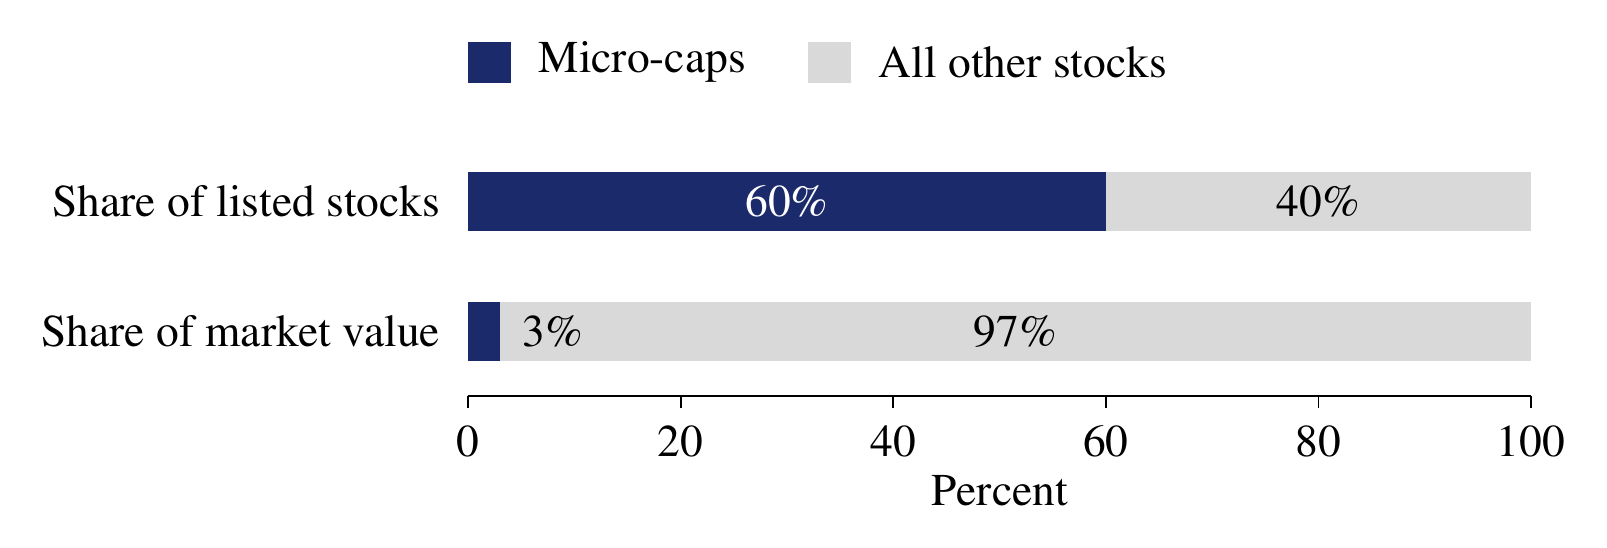
\includegraphics[width=0.8\linewidth]{images/fig02-3-microcaps.png}
%\caption{Micro-caps are most of the stocks but almost none of the money. Source: Fama and French (2008).}
%\label{fig:02-microcaps}
%\end{figure}


\providecolor{fenavy}{HTML}{1B2A6B}

\begin{figure}[!htbp]
  \centering
  \begin{tikzpicture}
  \begin{axis}[
    scale only axis, width=0.6\linewidth, height=2.4cm,
    xmin=0, xmax=100, ymin=0.4, ymax=2.6,
    axis x line*=bottom, axis y line=none,
    xtick={0,20,...,100},
    xlabel={Percent},
    xlabel style={yshift=4pt},
    clip=false,
  ]
    % Share of listed stocks: micro-caps 60%, others 40%
    \fill[fenavy]  (axis cs:0,1.7)  rectangle (axis cs:60,2.3);
    \fill[gray!25] (axis cs:60,1.7) rectangle (axis cs:100,2.3);
    \node[white] at (axis cs:30,2) {60\%};
    \node        at (axis cs:80,2) {40\%};

    % Share of market value: micro-caps 3%, others 97%
    \fill[fenavy]  (axis cs:0,0.7) rectangle (axis cs:3,1.3);
    \fill[gray!25] (axis cs:3,0.7) rectangle (axis cs:100,1.3);
    \node[anchor=west] at (axis cs:3.5,1) {3\%};
    \node              at (axis cs:51.5,1) {97\%};

    % Row labels
    \node[anchor=east] at (axis cs:-1,2) {Share of listed stocks};
    \node[anchor=east] at (axis cs:-1,1) {Share of market value};

    % Legend
    \fill[fenavy]  (axis cs:0,2.95)  rectangle (axis cs:4,3.25);
    \node[anchor=west] at (axis cs:5,3.1) {Micro-caps};
    \fill[gray!25] (axis cs:33,2.95) rectangle (axis cs:37,3.25);
    \node[anchor=west] at (axis cs:38,3.1) {All other stocks};
  \end{axis}
  \end{tikzpicture}
\caption{Micro-caps are most of the stocks but almost none of the money. Source: Fama and French (2008).}
\label{fig:02-microcaps}
\end{figure}


This matters because of the way portfolios are weighted (Section~\ref{sec:02-foundations}).

\begin{itemize}
  \item \textbf{Equal-weighted}\index{index weighting!equal-weighted|textbf} portfolios give every stock the same weight, so micro-caps dominate them simply because there are so many of them.
  \item \textbf{Value-weighted}\index{index weighting!value-weighted|textbf} portfolios weight stocks by market capitalization, so they reflect where investors' money actually is.
\end{itemize}

Micro-caps are also expensive and difficult to trade. Their \textbf{bid--ask spreads}\index{bid--ask spread|textbf}, the gap between the price at which you can buy and the price at which you can sell, are wide. They have little \textbf{liquidity}\index{liquidity|textbf}, which means that buying or selling even a modest amount moves the price. They are also costly to \textbf{sell short}\index{short selling|textbf}, that is, to borrow and sell in the hope of buying them back later at a lower price. In addition, micro-caps have the most extreme returns and the most data problems, including the missing delisting returns described in Section~\ref{sec:02-survivorship}. A pattern that appears in equal-weighted portfolios but not in value-weighted ones may therefore exist only where no large investor can exploit it.

The replication\index{replication} debate in Chapter~\ref{ch:10} turns partly on this point. An \textbf{anomaly}\index{anomaly|textbf} is a pattern in returns that standard risk models, such as the CAPM\index{capital asset pricing model (CAPM)}, cannot explain. Hou, Xue and Zhang\index{q-factor model} (2020) found that many anomalies disappear when micro-caps are given little weight, while their critics argue that this mainly shows that anomalies are concentrated among small stocks. Either way, the lesson for this chapter is simple: \textbf{always ask how a portfolio is weighted and whether the result survives without micro-caps.}

\begin{callout}
\textbf{What Failed: the size effect\index{size premium}.} Banz (1981) found that small companies had earned higher risk-adjusted returns than large ones, and ``small beats big'' became one of the best-known findings in finance. Later research, however, found that the effect became much weaker after it was published, that it was heavily concentrated among the very smallest stocks, and that in the early studies it was concentrated in January. Size remains a common factor in models of risk, but as a stand-alone source of extra return it has been far less reliable than its early evidence suggested. Lab~\ref{ch:02} tests how much of the size premium comes from micro-caps and how much comes from the years before 1981.
\end{callout}

\section{Data snooping: when a whole field searches one dataset}
\label{sec:02-snooping}

Chapter~\ref{ch:01} described the problem of selection within one researcher's search. There is a wider version of the same problem, in which an entire field searches the same data. Most research on U.S. stocks uses CRSP, and much of it uses the same period after 1963. Thousands of researchers have tested thousands of ideas on these data, and the ideas that ``worked'' were the ones that got published. Each paper may report a single, honest test, yet together the field has run an enormous number of trials on one history. A finding can therefore be a false discovery even when its author did nothing wrong, which is why a result must be confirmed on data that played no part in finding it.

Lo and MacKinlay (1990) called this \textbf{data-snooping bias}\index{data snooping|textbf}. When the choice of what to test is influenced by what earlier studies found in the same data, the usual significance levels\index{hypothesis testing!significance level} overstate the strength of the evidence. No single researcher can fix this bias, because no one knows how many ideas were tried and abandoned across the whole field.

Three defenses work, and later chapters use all of them.

\begin{enumerate}
  \item \textbf{New data.} Test the claim in periods or markets that played no part in its discovery, such as the years before the original sample, the years after publication, or other countries (Chapters~\ref{ch:08}--\ref{ch:10}).
  \item \textbf{Higher hurdles.} Require stronger evidence for claims that are tested on heavily used data, such as a t-statistic\index{t-statistic} above 3 (Harvey, Liu and Zhu 2016; Chapter~\ref{ch:10}).
    \item \textbf{Economic reasoning stated in advance.} Before running a test, state why the pattern should exist. A story written after a pattern is found proves little, because a clever explanation can be invented for almost any result, including one produced by chance. A reason stated beforehand turns the test into a genuine check, because the data can prove it wrong. 
\end{enumerate}

\section{Lab~\thechapter: Four ways data can mislead}
\label{sec:02-lab}

\begin{callout}
\textbf{Lab~\ref{ch:02} at a glance.} \emph{Claim on trial:} free, public data can support a reliable backtest. \emph{Data:} monthly and daily U.S. market returns and size-sorted portfolios\index{portfolio sort} since 1926, from the Kenneth R. French Data Library\index{Kenneth French data library} (downloaded automatically), plus a simulated stock market. \emph{Tools:} Python with pandas, NumPy and matplotlib, plus the fintest module. \emph{Time:} about 90 minutes, including the guided notebook. \emph{Code:} repository folder \texttt{ch02-data-traps/}.
\end{callout}

The design of this lab draws on a line of well-known studies, each of which showed how one feature of the data can change a result. Brown, Goetzmann, Ibbotson and Ross (1992) used a simulation to show that dropping the funds that disappear can create patterns in performance that are not really there, and Shumway (1997) measured how large the missing delisting losses are. Brock, Lakonishok and LeBaron (1992) made moving-average trading rules famous, and Sullivan, Timmermann and White (1999) later showed how much of their apparent success came from searching across many rules. Banz (1981) discovered the size effect, and Horowitz, Loughran and Savin (2000) and Schwert (2003) found that it weakened after publication and depended heavily on the smallest stocks. Each part of the lab follows the logic of one of these studies, using free data, so that you can see the problem for yourself.

The lab measures each of the problems from Sections~\ref{sec:02-returns} to~\ref{sec:02-microcaps} in turn. Three of its parts use real data, while the part on survivorship uses a simulation. 
The reason for the simulation is itself part of the lesson. To measure survivorship bias, we need to compare a backtest on all companies, including the ones that failed, with the same backtest on the survivors alone. Free stock-price sites list mainly the companies that still exist, so the failures are missing. The French library does include failed companies, but only inside its portfolio returns, so we cannot take them out to see how much difference they make. A simulation solves this problem, because it gives us the full history of every company, including the ones that disappear.



\subsection*{Part A: Arithmetic versus geometric averages}

\textbf{Predict first.} Before running this part, write down which of the four portfolios you expect to show the largest gap between its arithmetic and geometric average returns, and roughly how large you expect that gap to be.

The lab computes both averages for Treasury bills, the stock market, and the largest and smallest 10\% of stocks, annualizing each in the same way so that the comparison is fair. It then compares each measured gap with the volatility-drag approximation from Section~\ref{sec:02-returns}, which says that the geometric average is roughly the arithmetic average minus half the variance\index{variance}, $G \approx A - \sigma^2/2$ (Lab Figure~\ref{ch:02}.1). You should expect almost no gap for Treasury bills, a gap of about 2 percentage points a year for the market, and the largest gap, several points a year, for the smallest stocks. If a measured gap differs from the approximation, ask why. The approximation assumes that returns are close to normally distributed, and the returns of small stocks are not.

\subsection*{Part B: Survivorship bias in a market where the truth is known}

\textbf{Predict first.} Before running this part, write down how much you expect survivorship bias to add to the market's average return each year.

With real data we never know the true answer, so the lab builds a market in which we do. This approach follows Brown, Goetzmann, Ibbotson and Ross (1992), who simulated funds with no skill and showed that keeping only the survivors made their performance appear to persist. The lab simulates about 2,000 listed companies over 30 years, and every company has the \textbf{same expected return}, so no stock or strategy has a real advantage. Following Shumway (1997), a company whose price falls below 20\% of its listing price is delisted with a final return of $-30$\%. Other companies are acquired at a premium, and every company that leaves is replaced by a new listing.

From this single simulated history, the lab builds three datasets:

\begin{center}
\small
\begin{tabularx}{0.9\linewidth}{@{}>{\raggedright\arraybackslash}p{0.26\linewidth}>{\raggedright\arraybackslash}X>{\raggedright\arraybackslash}p{0.28\linewidth}@{}}
\toprule
Dataset & What it contains & Real-world equivalent \\
\midrule
Full data & Every company, including its delisting return & CRSP, used correctly \\
Missing delisting returns & Every company, but without the final delisting month & A database with gaps in delisting returns \\
Survivors only & Only companies still listed at the end & Today's stocks downloaded from a free price site \\
\bottomrule
\end{tabularx}
\end{center}

On each dataset, the lab measures two things. The first is the equal-weighted market return. The second is the return of a strategy that each month buys the most volatile fifth of stocks and sells the least volatile fifth, where volatility is measured using past returns only (Lab Figure~\ref{ch:02}.2). The full data give the true answer, so any difference in the other two datasets comes entirely from the way they were built.

With the lab's default settings (2,000 listed companies, 30 years and seed 2026), 5,856 companies are listed over the period, 1,693 of them are delisted for poor performance, and 2,000 survive to the end. The results are as follows:

\begin{center}
\small
\begin{tabularx}{0.9\linewidth}{@{}>{\raggedright\arraybackslash}X>{\raggedright\arraybackslash}p{0.22\linewidth}>{\raggedright\arraybackslash}p{0.22\linewidth}r@{}}
\toprule
Dataset & Equal-weighted compound return & Volatile minus calm, per year & t-statistic \\
\midrule
Full data & 9.3\% & $-1.2$\% & $-2.2$ \\
Missing delisting returns & 10.7\% & $+2.0$\% & 3.5 \\
Survivors only & 14.0\% & $+12.0$\% & 14.7 \\
\bottomrule
\end{tabularx}
\end{center}

Read the table from top to bottom. In the full data, the volatile-minus-calm strategy loses about 1\% a year, because volatile companies are delisted more often. Leaving out only the delisting returns flips the sign, so that the strategy now appears to earn 2\% a year. Keeping only the survivors adds almost five percentage points a year to the market's return and creates a ``volatility premium'' of 12\% a year, with a t-statistic far beyond any hurdle in this book. None of this premium is real. Compare these numbers with your prediction.

\subsection*{Part C: Look-ahead bias}

\textbf{Predict first.} Before running this part, write down whether you expect a one-day timing error to change a strategy's Sharpe ratio a little or a lot.

\textbf{C1. Trading on the same day's close.} This part tests a classic timing rule, which holds stocks when the market closes above its 200-day \textbf{moving average}\index{moving average|textbf}, the average closing price over the past 200 trading days, and holds Treasury bills otherwise. Brock, Lakonishok and LeBaron (1992) studied rules of this kind on nearly a century of daily Dow Jones data and found that they appeared to predict returns. The lab runs the rule in two ways. The correct version makes its decision at yesterday's close and earns today's return, whereas the look-ahead version makes its decision at today's close but is still credited with today's return. The two versions differ by a single day, which is the kind of error that can hide in one misplaced line of code. Compare their returns and Sharpe ratios (Lab Figure~\ref{ch:02}.3).

\textbf{C2. Choosing the window with hindsight.} Next, the lab tests moving-average windows from 20 to 300 days and chooses one of them in two ways. The hindsight version picks the window with the best Sharpe ratio over the whole evaluation period. The walk-forward version picks, each January, the window that had worked best up to that point, using only past data (Lab Figure~\ref{ch:02}.4). The gap between the two versions measures how much a result is inflated by choosing a rule's settings after seeing the results. Sullivan, Timmermann and White (1999) made the same point on a much larger scale. They expanded the rules of Brock, Lakonishok and LeBaron to a universe of several thousand and adjusted for the search with a bootstrap\index{bootstrap}. The best rule still looked strong in the original sample, but it did not continue to outperform in the decade that followed.

\subsection*{Part D: Micro-caps, weighting and the size premium}

\textbf{Predict first.} Before running this part, write down whether you expect the size premium to be larger in value-weighted or in equal-weighted portfolios, and whether you expect it to survive after 1981.

Using size-sorted portfolios, the lab measures the \textbf{size premium}\index{size premium|textbf}, which is the return of the smallest tenth of stocks minus the return of the largest tenth. It does so in four ways, using value weights and equal weights, each with and without the smallest tenth of stocks. It then splits the sample into the years before and after Banz published his finding in 1981 (Lab Figure~\ref{ch:02}.5). Together, these steps test the What Failed box in Section~\ref{sec:02-microcaps} directly. They also repeat, with free data, two tests from the literature. Horowitz, Loughran and Savin (2000) found that removing the very smallest firms eliminated any statistically significant\index{statistical significance} size effect, and Schwert (2003) found that the size effect weakened after the papers that reported it were published. If the premium lives mainly in tiny, hard-to-trade stocks, or if it disappeared after it was published, the claim weakens.

\emph{[Draft note: figures and numbers for Parts A, C and D are generated from the Kenneth R. French data at the time of publication; the book prints those results. The Part B simulation is fixed by design and its results can be printed as they stand.]}

\subsection*{Your verdict}

Readers write one sentence for each problem, saying how much it changed the result and in which direction, and then judge the claim. The expected verdict is \textbf{survives, with conditions}. Free data can support a reliable backtest when you do the following:

\begin{enumerate}
  \item use total returns, compare them with a total-return benchmark, and quote the geometric average when reporting growth (Part A);
  \item use data that include failed companies, such as the French library's portfolios, which are built from CRSP, rather than a list of today's stocks (Part B);
  \item lag every signal and every accounting figure, and choose a rule's settings with walk-forward tests (Part C);
  \item check that the result survives value weighting and the removal of micro-caps (Part D).
\end{enumerate}

A backtest that skips these steps can look excellent and still mean nothing, while one that follows them can be trusted as far as its statistics allow. The checklist in the next section turns these conditions into questions that you can ask of any backtest, including your own.

\section{What investors can use: a data checklist}
\label{sec:02-checklist}

Before you trust any backtest, whether it is your own or someone else's, work through the following questions. Each question corresponds to a section of this chapter, and most of them can be answered in a few minutes.

\begin{itemize}
  \item[$\square$] \textbf{Returns (Section~\ref{sec:02-returns}):} Are the returns total returns that include dividends? Are they compared with a total-return benchmark? Is the reported average arithmetic or geometric?
  \item[$\square$] \textbf{Excess returns (Section~\ref{sec:02-returns}):} Is performance measured above the risk-free rate?
  \item[$\square$] \textbf{Survivorship (Section~\ref{sec:02-survivorship}):} Does the dataset include companies or funds that no longer exist, and are their delisting returns included?
  \item[$\square$] \textbf{Look-ahead (Section~\ref{sec:02-lookahead}):} Is every signal lagged so that it uses only information available before the trade, and are accounting data lagged to their publication dates?
  \item[$\square$] \textbf{Hindsight choices (Section~\ref{sec:02-lookahead}):} Were any parameters, thresholds or universes chosen using the whole sample?
  \item[$\square$] \textbf{Weighting (Section~\ref{sec:02-microcaps}):} Is the portfolio value-weighted or equal-weighted, and does the result survive without micro-caps?
  \item[$\square$] \textbf{Shared data (Section~\ref{sec:02-snooping}):} Has the result been tested on data that played no part in its discovery, such as other periods, other markets or the years after publication?
\end{itemize}

\textbf{Questions to ask a fund manager or strategy vendor}

\begin{itemize}
  \item Which database was the backtest built on, and does it include delisted stocks and their delisting returns?
  \item How were the signals lagged, and when would each piece of data actually have been available?
  \item Is the strategy value-weighted or equal-weighted, and what share of its return comes from the smallest stocks?
  \item Is the reported return an arithmetic or a compound average, and is it measured before or after costs?
\end{itemize}

\section*{Exercises}
\addcontentsline{toc}{section}{Exercises}

\subsection*{Conceptual (all readers)}

\begin{enumerate}
  \item A strategy reports an average annual return of 18\% with a volatility of 40\%. Estimate its geometric average. Which number should an investor care about, and why?
  \item Explain why a portfolio's simple return is a weighted average of the simple returns of its holdings, while a multi-period return is a sum of log returns.
  \item A researcher backtests a strategy from 2005 to today on the stocks that are in the S\&P 500 index today. Name two biases in this design and the direction of each.
  \item A study uses annual accounting data for fiscal years ending in December and forms portfolios in January of the next year. What is the problem, and how do Fama and French avoid it?
  \item Explain why survivorship bias can create a premium for volatile stocks, rather than simply raising all returns by the same amount.
  \item A paper reports a strong anomaly in equal-weighted portfolios that disappears in value-weighted ones. What does this suggest about who could profit from it?
\end{enumerate}

\subsection*{Lab extensions (technical readers)}

\begin{enumerate}
  \setcounter{enumi}{6}
  \item Re-run Part B with a delisting return of $-55$\%, which is closer to the estimates for Nasdaq stocks. How do the three datasets change?
  \item In Part C, try windows of 50 and 300 days. Is the look-ahead gain larger for fast rules or for slow ones? Explain why.
  \item In Part C, charge a trading cost of 0.1\% each time the rule switches. Does the correctly traded rule still beat buy-and-hold on a risk-adjusted basis?
  \item In Part D, move the publication split to 1990 and then to 2000. When does the size premium appear to fade?
  \item \textbf{Challenge:} Using a free price source, backtest an equal-weighted portfolio of today's S\&P 500 members over the past 20 years and compare it with the equal-weighted S\&P 500 index. Which problem from this chapter explains the difference?
\end{enumerate}
